\documentclass[tikz,border=10pt]{standalone}
\usepackage{tkz-euclide} % 增强几何绘图功能
\usetikzlibrary{calc, intersections}

\begin{document}
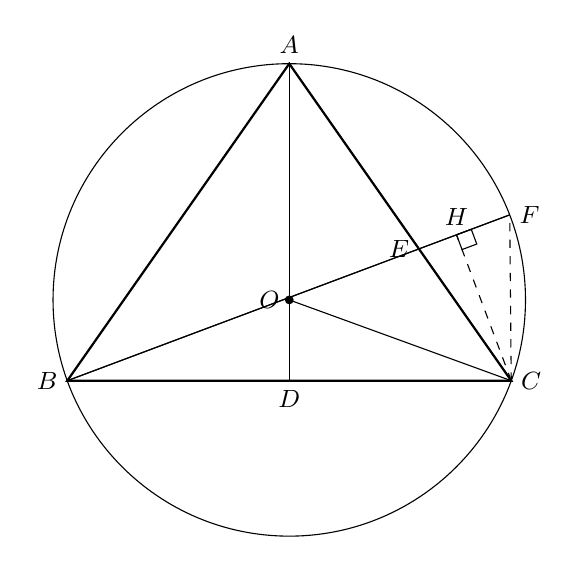
\begin{tikzpicture}[scale=2, font=\small]
    % 1. 定义圆心 O 和半径
    \coordinate (O) at (0,0);
    \def\R{1.5}
    \draw (O) circle (\R);
    \fill (O) circle (0.8pt) node[left] {$O$};

    % 2. 定义顶点 A, B, C (根据图像比例设定角度)
    \coordinate (A) at (90:\R);
    \coordinate (B) at (200:\R);
    \coordinate (C) at (-20:\R);

    % 3. 连接三角形线段
    \draw[thick] (A) -- (B) -- (C) -- cycle;

    % 4. 线段 AD (A 到 BC 的垂线)
    \coordinate (D) at ($(B)!(A)!(C)$);
    \draw (A) -- (D);
    \node[below] at (D) {$D$};

    % 5. 射线 BF 过 O 点交 AC 于 E，交圆于 F
    \coordinate (F) at (1.4,0.54);
    \draw (B) -- (F);           % 实线 BF
    \draw[name path=lineBF] (B) -- (F); 
    \draw[name path=lineAC] (A) -- (C);
    \path [name intersections={of=lineBF and lineAC, by=E}];
    \draw (O) -- (C);           % 连线 OC
    
    % 6. 辅助线与垂足 H (过 C 作 BF 的垂线)
    \coordinate (H) at ($(B)!(C)!(F)$);
    \draw[dashed] (C) -- (H);   % 辅助线用虚线表示
    \draw[dashed] (C) -- (F); 
    % 7. 标注点
    \node[above] at (A) {$A$};
    \node[left] at (B) {$B$};
    \node[right] at (C) {$C$};
    \node[right] at (F) {$F$};
    \node[left] at (E) {$E$};
    \node[above] at (H) {$H$};

    % 8. 绘制直角标记
    \tkzMarkRightAngle[size=0.1](C,H,F)

\end{tikzpicture}
\end{document}